%%%%%%%%%%%%%%%%%%%%%%%%%%%%%%%%%%%%%%%%%
% University/School Laboratory Report
% LaTeX Template
% Version 3.1 (25/3/14)
%
% This template has been downloaded from:
% http://www.LaTeXTemplates.com
%
% Original author:
% Linux and Unix Users Group at Virginia Tech Wiki 
% (https://vtluug.org/wiki/Example_LaTeX_chem_lab_report)
%
% License:
% CC BY-NC-SA 3.0 (http://creativecommons.org/licenses/by-nc-sa/3.0/)
%
% Modified for Design (E) 314 Report by Arno Barnard, title page adapted from UCT Report Template
% Further modified for Design (E) 344 by Coenrad Fourie
%%%%%%%%%%%%%%%%%%%%%%%%%%%%%%%%%%%%%%%%%

%----------------------------------------------------------------------------------------
%	PACKAGES AND DOCUMENT CONFIGURATIONS
%----------------------------------------------------------------------------------------

\documentclass[11pt,a4paper]{article}

\usepackage{geometry} % To set page size and margins accurately
\usepackage[version=3]{mhchem} % Package for chemical equation typesetting
\usepackage{siunitx} % Provides the \SI{}{} and \si{} command for typesetting SI units
\usepackage{graphicx} % Required for the inclusion of images
%\usepackage{natbib} % Required to change bibliography style to APA
\usepackage{amsmath} % Required for some math elements 
\usepackage{paralist} % For compactitem lists
\usepackage{color} % Color management options
\usepackage{listings} % To typeset source code
\usepackage{pdflscape} % Landscape pages
\usepackage{acro} %To create acronyms lists
\usepackage{hyperref} % Clickable links
\usepackage{minted} % Syntax highlighting for code
\usepackage{float}
\usepackage{fancyhdr}
\usepackage{caption} 
\usepackage{url}
\usepackage{hyperref}
\usepackage{pdfpages}

\usepackage[acronym]{glossaries}
\geometry{
a4paper,
total={170mm,257mm},
left=20mm,
top=20mm,
}
\setlength\parindent{0.5cm} % Set indentation for paragraphs
% To make floats, on float only pages, placed at top.
\makeatletter
\setlength{\@fptop}{0pt}
\setlength{\@fpbot}{0pt plus 1fil}
\makeatother
%\renewcommand{\labelenumi}{\alph{enumi}.} % Make numbering in the enumerate environment by letter rather than number (e.g. section 6)

%----------------------------------------------------------------------------------------
%	ACRONYMS AND SYMBOLS
%----------------------------------------------------------------------------------------
% abbreviations:
\DeclareAcronym{ny}{
short = NY ,
long  = New York ,
tag = abbrev
}
\DeclareAcronym{cpu}{
short = CPU ,
long  = central processing unit ,
short-plural = s ,
long-plural = s ,
tag = abbrev
}
\DeclareAcronym{un}{
short = UN ,
long  = United Nations ,
tag = abbrev
}
\DeclareAcronym{lcd}{
short = LCD ,
long  = Liquid Crystal Display ,
tag = abbrev
}

% symbols
\DeclareAcronym{angelsperarea}{
short = \ensuremath{a} ,
long  = The number of angels per unit area ,
sort = a ,
tag = symbol
}
\DeclareAcronym{numofangels}{
short = \ensuremath{N} ,
long  = The number of angels per needle point ,
sort = N ,
tag = symbol
}
\DeclareAcronym{areaofneedle}{
short = \ensuremath{A} ,
long  = The area of the needle point ,
sort = A ,
tag = symbol
}

%----------------------------------------------------------------------------------------
%	DOCUMENT INFORMATION AND TITLE PAGE
%----------------------------------------------------------------------------------------

\title{Analogue Signal Generator} % Title

\author{Benjamin Frederick Johannnes KROG \textsc{}} % Author name

\date{\today} % Date for the report

\makeatletter
\let\thetitle\@title
\let\theauthor\@author
\let\thedate\@date
\makeatother

%\pagestyle{fancy}
%\fancyhf{}
%\rhead{\theauthor}
%\lhead{\thetitle}
%\cfoot{\thepage}

\begin{document}

\begin{titlepage}
    \centering
    \vspace*{0.5 cm}
    
\includegraphics[scale = 1.5]{SU_logo_RGB-01.png}\\[1.0 cm]   % University Logo
    \textsc{\LARGE Design (E) 344 \\ Technical Report}\\[0.5 cm]               % Course Name
    \rule{\linewidth}{0.2 mm} \\[0.4 cm]
    { \huge \bfseries \thetitle }\\[0.4 cm]
    \rule{\linewidth}{0.2 mm} \\[1.5 cm]
    
    \begin{minipage}{6.5cm}
    	\begin{flushleft} \large
    		\emph{Author:}\\
    		\theauthor
    	\end{flushleft}
    \end{minipage}~
    \begin{minipage}{6.5cm}
    	\begin{flushright} \large
    		\emph{Student Number:} \\
    		{27163296}                                 % Your Student Number
    	\end{flushright}
    \end{minipage}\\[2 cm]
    
    {\large \thedate}\\[2 cm]
    
    \vfill
    
\end{titlepage}

%----------------------------------------------------------------------------------------
%	DECLARATION - DUAL LANGUAGE
%----------------------------------------------------------------------------------------
{\Large \bf Plagiaatverklaring / Plagiarism Declaration}
\begin{enumerate}
    \item Plagiaat is die oorneem en gebruik van die idees, materiaal en ander intellektuele eiendom van ander persone asof dit jou eie werk is.\\
    \textit{Plagiarism is the use of ideas, material and other intellectual property of another's work and to present is as my own.}
    \item Ek erken dat die pleeg van plagiaat 'n strafbare oortreding is aangesien dit 'n vorm van diefstal is. \\
    \textit{I agree that plagiarism is a punishable offence because it constitutes theft.}
    \item Ek verstaan ook dat direkte vertalings plagiaat is.\\
    \textit{I also understand that direct translations are plagiarism.}
    \item Dienooreenkomstig is alle aanhalings en bydraes vanuit enige bron (ingesluit die internet) volledig verwys (erken). Ek erken dat die woordelikse aanhaal van teks sonder aanhalingstekens (selfs al word die bron volledig erken) plagiaat is.\\
    \textit{Accordingly all quotations and contributions from any source whatsoever (including the internet) have been cited fully. I understand that the reproduction of text without quotation marks (even when the source is cited) is plagiarism.}
    \item Ek verklaar dat die werk in hierdie skryfstuk vervat, behalwe waar anders aangedui, my eie oorspronklike werk is en dat ek dit nie vantevore in die geheel of gedeeltelik ingehandig het vir bepunting in hierdie module/werkstuk of 'n ander module/werkstuk nie.\\
    \textit{I declare that the work contained in this assignment, except where otherwise stated, is my original work and that I have not previously (in its entirety or in part) submitted it for grading in this module/assignment or another module/assignment.}
\end{enumerate}
\vspace{1cm}
\begin{table}[ht]
	\begin{center}
		\begin{tabular*}{15.5cm}{@{\extracolsep{\fill}}lll}
			%		\begin{tabular}{l l l}
				
\includegraphics[width=0.25\textwidth]{figures/signature2.png} & & \text{27163296} \\
				\makebox[8cm]{\hrulefill} & & \makebox[6cm]{\hrulefill}\\
				Handtekening / \textit{Signature} & & Studentenommer / \textit{Student number}\\[1cm]
				\text{BFJ KROG} & & \text{23 Oct 2025} \\
				\makebox[8cm]{\hrulefill} & & \makebox[6cm]{\hrulefill}\\ 
				Voorletters en van / \textit{Initials and surname} & & Datum / \textit{Date} \\
			\end{tabular*}
		\end{center}
	\end{table}
	\newpage

%----------------------------------------------------------------------------------------
%	ABSTRACT
%----------------------------------------------------------------------------------------
\begin{abstract}
    This will be where you write your abstract, e.g.:
    
    An analogue signal generator with square, triangle and sine wave output was developed. This report\ldots
\end{abstract}
\newpage

%----------------------------------------------------------------------------------------
%	TOC, Lists (Figures, Tables etc)
%----------------------------------------------------------------------------------------
\tableofcontents
\listoffigures
\listoftables

%Acronym lists
\printacronyms[include = abbrev, name = {List of Abbreviations}]
\printacronyms[include = symbol, name = {List of Symbols}]
\newpage

%----------------------------------------------------------------------------------------
%	SECTION 1
%----------------------------------------------------------------------------------------
\section{Introduction}
Here you describe your overall project briefly, context, specifications, limitations, aims etc. Please note that this is a template, and you can add subsections as you require.

Take great care to reference sources when ideas from publications, textbooks, internet sources and more are used during your design process.


%----------------------------------------------------------------------------------------
%	SECTION 2
%----------------------------------------------------------------------------------------
\section{System description}\label{sec:desc}
Here you will describe your system. Be sure to include a system diagram, and reference it, for instance, as: The system diagram is shown in Figure~\ref{fig:place}. An external regulated power supply provides a single supply voltage of +\SI{30}{\volt} to the system. The output to the load is from a BNC socket\ldots
dq

%----------------------------------------------------------------------------------------
%	SECTION 3
%----------------------------------------------------------------------------------------
\newpage
\section{Hardware design and implementation}
Describe hardware design and verification with SPICE simulation in this section. When equations are used, these must be place (and numbered) as follows:

%----------------------------------------------------------------------------------------
\subsection{Hardware block diagram and description of interaction}

\begin{figure}[H]
	\centering
	\begin{minipage}{0.8\textwidth}
		\centering
		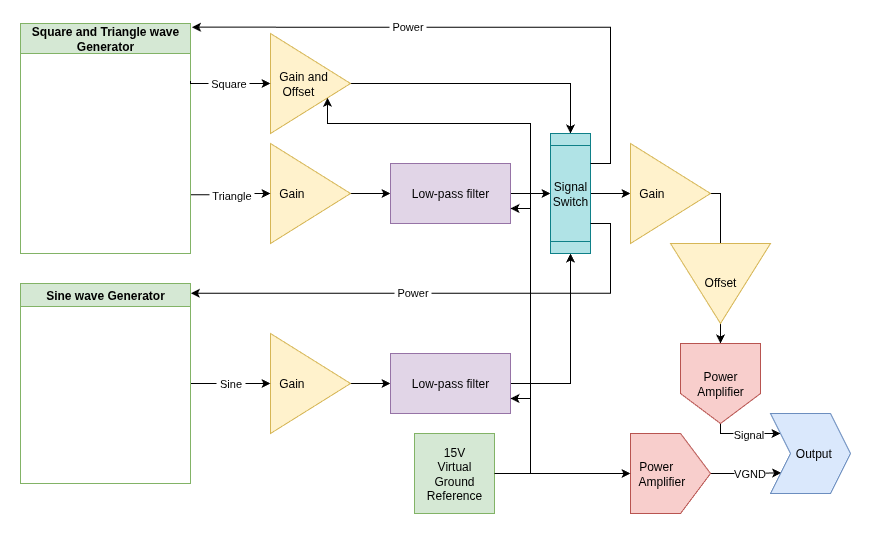
\includegraphics[width=1\textwidth]{figures/hardware/hardware-design-overview-block-diagram.drawio.png}
		\caption{Hardware design overview block diagram}
		\label{fig:Hardware design overview block diagram}\textsf{}
	\end{minipage}
\end{figure}


Briefly describe the subsystems, and how each is connected to other subsystems in the full system.

%----------------------------------------------------------------------------------------
\subsection{Square wave generator}

Describe the square wave generator design, circuit diagram, frequency adjustment, pulse-width modulation adjustment, frequency range selection and any other relevant design steps (such as the use of dual pots to control frequency while keeping duty cycle constant).

%----------------------------------------------------------------------------------------
\subsection{Triangle wave generator}

Describe the triangle wave generator design, circuit diagram, frequency adjustment (if different from the square wave), frequency range selection, skew adjustment and any other relevant design steps (for instance: how to keep frequency constant as skew is adjusted).

%----------------------------------------------------------------------------------------
\subsection{Sine wave generator}

Describe the sine wave generator design, circuit diagram, frequency adjustment, frequency range selection and any measures taken to guarantee a very low THD.

%----------------------------------------------------------------------------------------
\subsection{Summing, signal selection and Level adjustment}

\begin{figure}[H]
	\begin{center}
		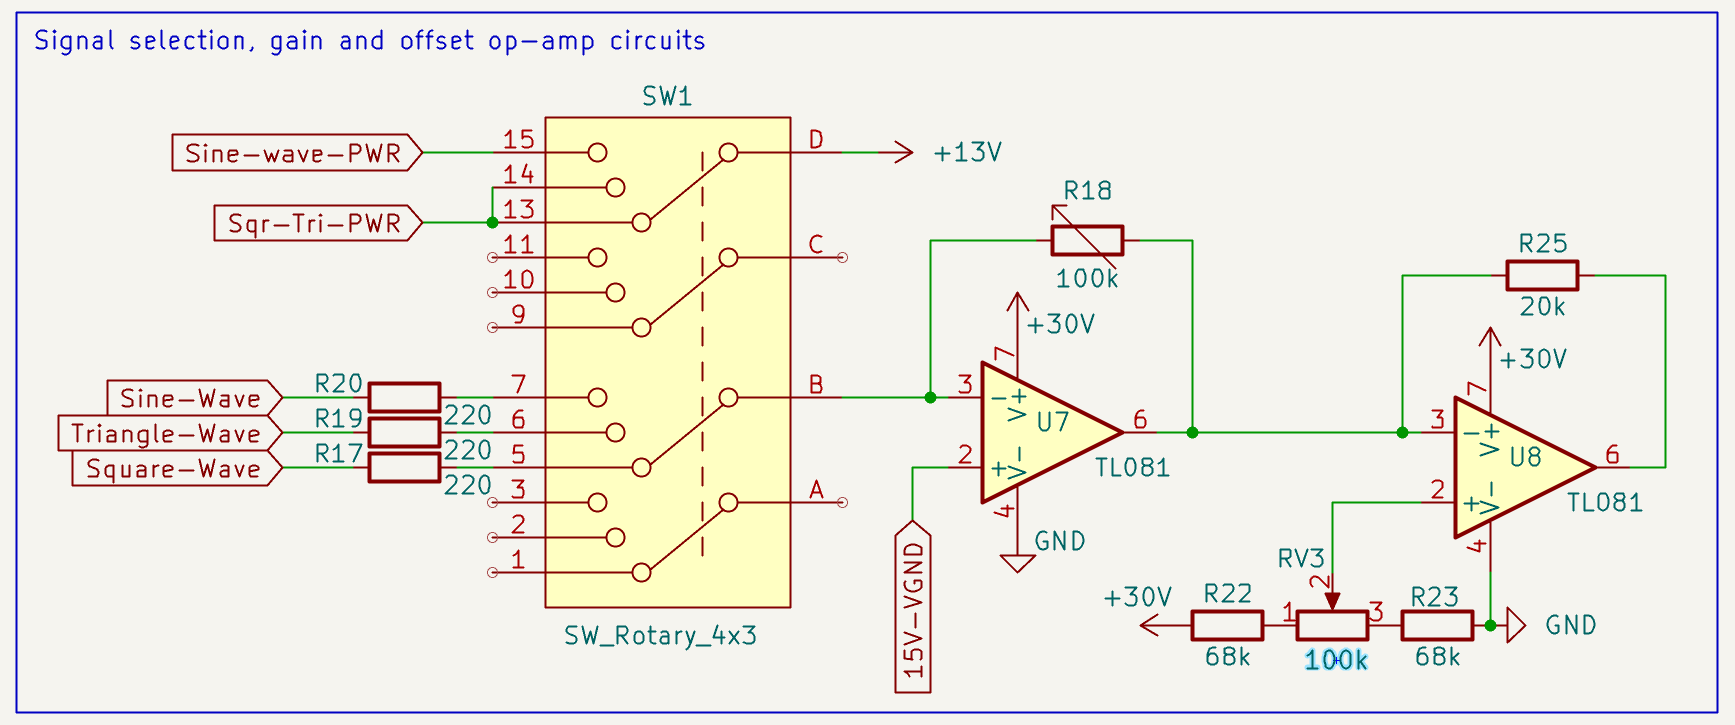
\includegraphics[width=0.9\textwidth]{figures/hardware/schematics/signal-gain-offset-op-amp-circuits.png}
		\caption{Signal selection, gain and offset op-amp circuits}
		\label{fig:Signal selection, gain and offset op-amp circuits}
	\end{center}
\end{figure}

Describe the design and circuit diagram of level adjustment functionality.

Describe the design and circuit diagram of the signal selection switch, pathways and gain matching resistors.


%----------------------------------------------------------------------------------------
\subsection{Full push-pull Amplifier}

\begin{figure}[H]
	\begin{center}
		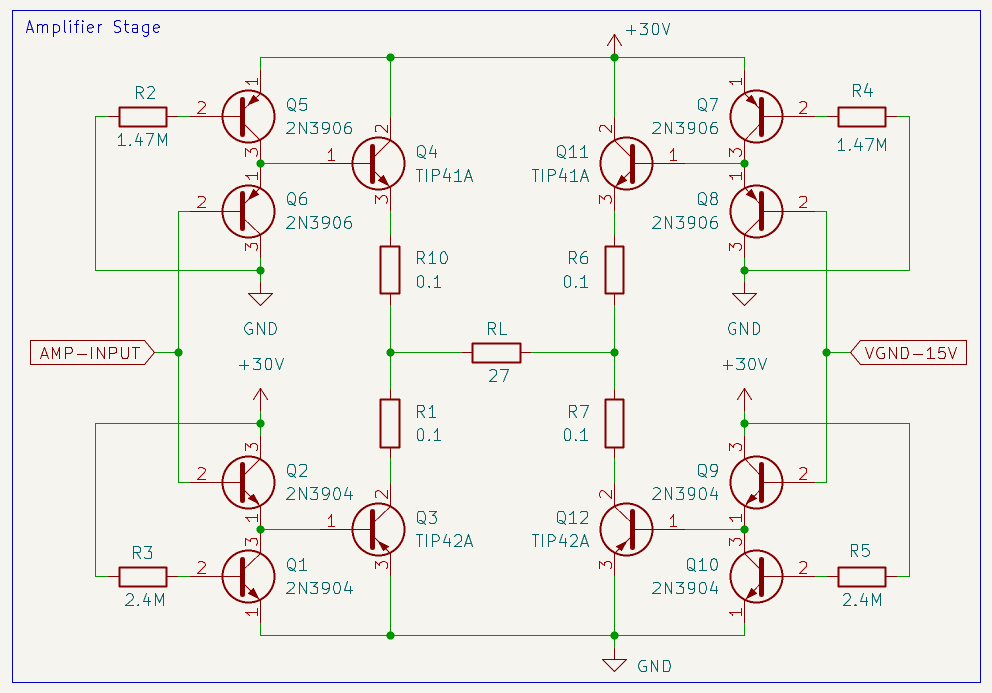
\includegraphics[width=0.9\textwidth]{figures/hardware/schematics/amplifier-circuit.png}
		\caption{Full push-pull amplifier circuit}
		\label{fig:full-push-pull-amplifier-circuit}
	\end{center}
\end{figure}


Describe the design and circuit diagram of the amplification stage to meet the signal amplitude adjustment requirements.

%----------------------------------------------------------------------------------------
\subsection{Voltage regulation, virtual ground and output drive capability}

Describe the design of any voltage regulation circuitry, the virtual ground and the driver design to meet the output source and sink current requirements. Include circuit schematics.

%----------------------------------------------------------------------------------------
\subsection{Other}

If you have other subsystems, add these.

%----------------------------------------------------------------------------------------
\subsection{Construction}

Discuss the construction of the system, from selection of component placement, to grounding, decoupling, input/output accessibility, packaging, etc. Include photographs of the final system.



%----------------------------------------------------------------------------------------
%	SECTION 4
%----------------------------------------------------------------------------------------
\newpage
\section{Software design and implementation}

Discuss top-level software design and implementation, using design tools, like flow diagrams where needed. 

%----------------------------------------------------------------------------------------
\subsection{Programming language}

Python was chosen as the language of choice for this  project for its vast library support, simple syntax and the fact that modern LLMs are able to understand and write python very well with few mistakes.  The draw backs of Python are that it is an interpreted language requiring a runtime making the final binary very large for a simple program. 
\newline \newline
mention pyinstaller
 \newline \newline
Discuss the selected programming language, the motivation for this selection, and the advantages and disadvantages of the selected programming language. 

%----------------------------------------------------------------------------------------
\subsection{Software block diagram and description of interaction}

\begin{figure}[H]
	\begin{center}
		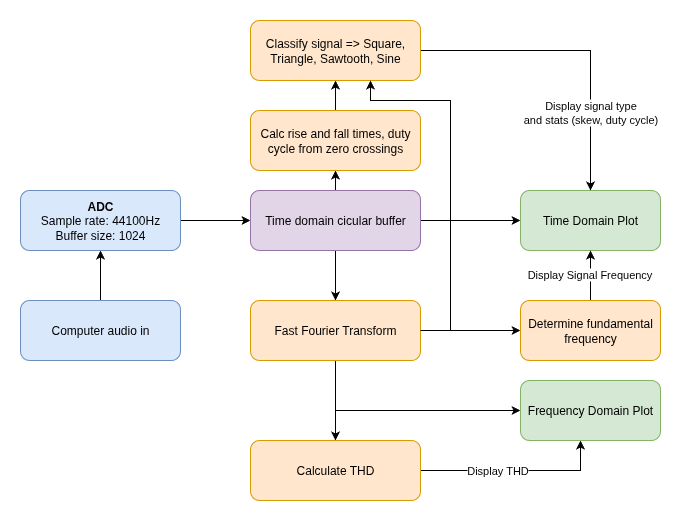
\includegraphics[width=0.75\textwidth]{figures/software/software-design-overview-block-diagram.png}
		\caption{Software design overview block diagram}
		\label{fig:Software design overview block diagram}
	\end{center}
\end{figure}


Describe the code functionality by block diagram.

%----------------------------------------------------------------------------------------
\subsection{Use of AI tools}

Describe any use of AI tools to generate sections of the software. Include a discussion on prompting the AI, as well as verifying the correctness and robustness of AI generated code.

%----------------------------------------------------------------------------------------
\subsection{Data read-in and calibration}

Describe read-in of measurements, especially in terms of how data is read in through a computer’s audio input, how it is calibrated and displayed.

%----------------------------------------------------------------------------------------
\subsection{Software functions}

Describe and show results for functions such as amplitude measurement, duty cycle/skew determination, frequency analysis (FFT), total harmonic distortion calculation, etc.

%----------------------------------------------------------------------------------------
%	SECTION 5
%----------------------------------------------------------------------------------------
\newpage
\section{Measurements and Results}

Describe your measurements and results to determine where your system meets or does not meet the requirements/specifications. Show the results by selected subsystem, as well as for the complete system. 

%----------------------------------------------------------------------------------------
\subsection{Square, triangle and sine waves}

Show oscilloscope measurements at the output of the system into a \SI{27}{\ohm} load if possible at \SI{100}{\hertz}, \SI{1}{\kilo\hertz} and \SI{10}{\kilo\hertz}, for \SI{10}{\volt} peak amplitude. Discuss the load resistance and the output current achieved. Analyse the results and discuss shortcomings. Specifically show how the single supply voltage is handled, and measure any characteristics necessary to demonstrate that the virtual ground and the output drivers (source/sink) function as designed.

%----------------------------------------------------------------------------------------
\subsection{Duty cycle and skew}

Show duty cycle and skew at the required limits (10\% to 90\%, or 0.1 to 10) at representative frequencies. Analyse and discuss. Compare oscilloscope measurements with those from your own software to validate the software and the circuit results.

%----------------------------------------------------------------------------------------
\subsection{Sine wave total harmonic distortion}

Measure the THD for the sine wave with your software if possible, and present FFT plots. Analyse and discuss results.

%----------------------------------------------------------------------------------------
\subsection{Level adjust}

Measure and discuss the level adjustment capability.

%----------------------------------------------------------------------------------------
\subsection{Other}

Any other measurements or subsystem characterisation unique to your system.


%----------------------------------------------------------------------------------------
%	SECTION 6
%----------------------------------------------------------------------------------------
\newpage
\section{Conclusions}
Use experimental results, design limitations and system performance, explain your conclusions drawn.

Use experimental results, design limitations and system performance, explain your conclusions drawn.
Highlight noise, oscillations and mitigation. Discuss signal quality (harmonic distortion).
Do not forget to reference ALL REFERENCES in text using IEEE Documentation Style~\cite{IEEErefguide:2023}.
All applicable documents should be in references list, specifically datasheets and application notes \cite{lm555:2014} used as references for designs, explanations of device operation etc.



\clearpage % So we get new page even after float flow-over

%----------------------------------------------------------------------------------------
%	BIBLIOGRAPHY
%----------------------------------------------------------------------------------------
\bibliographystyle{IEEEtran}
\bibliography{IEEEabrv,references}

%----------------------------------------------------------------------------------------

\end{document}